\title{Cantilever Beam Analytical Solution}
\author{
        Admir Makas \\
        Daniel Clark \\
        John Neiferd \\
}
%\date{\today}

\documentclass[12pt]{article}

\usepackage[T1]{fontenc} % Use 8-bit encoding that has 256 glyphs
\usepackage{fourier} % Use the Adobe Utopia font for the document - comment this line to return to the LaTeX default
\usepackage[english]{babel} % English language/hyphenation
\usepackage{amsmath,amsfonts,amsthm} % Math packages

\usepackage{sectsty} % Allows customizing section commands
\allsectionsfont{\centering \normalfont\scshape} % Make all sections centered, the default font and small caps

\usepackage{graphicx}

\usepackage[a4paper,lmargin=2.5 cm,rmargin=2 cm,tmargin=2 cm,bmargin=2 cm]{geometry}

\usepackage{fancyhdr} % Custom headers and footers
\pagestyle{fancyplain} % Makes all pages in the document conform to the custom headers and footers
\fancyhead{} % No page header - if you want one, create it in the same way as the footers below
\fancyfoot[L]{} % Empty left footer
\fancyfoot[C]{} % Empty center footer
\fancyfoot[C]{\thepage} % Page numbering for right footer
\renewcommand{\headrulewidth}{0pt} % Remove header underlines
\renewcommand{\footrulewidth}{0pt} % Remove footer underlines
\setlength{\headheight}{13.6pt} % Customize the height of the header

\usepackage{chngcntr}
%\numberwithin{equation}{section} % Number equations within sections (i.e. 1.1, 1.2, 2.1, 2.2 instead of 1, 2, 3, 4)
%\numberwithin{figure}{section} % Number figures within sections (i.e. 1.1, 1.2, 2.1, 2.2 instead of 1, 2, 3, 4)
%\counterwithout{figure}{section}
%\numberwithin{table}{section} % Number tables within sections (i.e. 1.1, 1.2, 2.1, 2.2 instead of 1, 2, 3, 4)

\setlength\parindent{0pt} % Removes all indentation from paragraphs - comment this line for an assignment with lots of text

\usepackage{amsmath}
\usepackage{float} % To firce the location of figure
\usepackage{subfigure} %For side-by-side figures
\usepackage{lettrine}
%\usepackage{lipsum}
\usepackage{epstopdf} %To read *.eps Files
\usepackage{listings} % To include source codes in LATEX document
\usepackage{mathrsfs} % To include script fonts. use \mathscr{}
\usepackage{courier} % To write in courier fornt
\usepackage{mathtools} % For mat symbols
\usepackage{xfrac} % For \sfrac{}{}
%\usepackage{subcaption}
\usepackage{booktabs} % To thicken table lines
%====================================================================================
\begin{document}
\maketitle

\section{Analytic Results}

\paragraph{}
Fourth order PDE for the Euler-Bernoulli was solved to obtain natural frequencies and mode shapes for the clampled-free boundary condition (CANTILEVER BEAM). First 10 natural frequencies are listed below and compared to FE results using ABAQUS. 

% Table generated by Excel2LaTeX from sheet 'Sheet1'
\begin{table}[H]
  \centering
  \caption{Beam Frequencies}
    \begin{tabular}{crrc}
    \toprule
    \multicolumn{4}{c}{\textbf{First 8 Natural Frequencies}} \\
    \midrule
    \textbf{Mode} & \textbf{Analytical Resuls} & \textbf{ABAQUS Results} & \textbf{\% Error} \\
    1     & \multicolumn{1}{c}{0.0263} & \multicolumn{1}{c}{0.0261} & 0.7\% \\
    2     & \multicolumn{1}{c}{0.1647} & \multicolumn{1}{c}{0.1615} & 1.9\% \\
    3     & \multicolumn{1}{c}{0.4613} & \multicolumn{1}{c}{0.4485} & 2.8\% \\
    4     & \multicolumn{1}{c}{0.9039} & \multicolumn{1}{c}{0.8749} & 3.2\% \\
    5     & \multicolumn{1}{c}{1.4942} & \multicolumn{1}{c}{1.4449} & 3.3\% \\
    6     & \multicolumn{1}{c}{2.2321} & \multicolumn{1}{c}{2.1505} & 3.7\% \\
    7     & \multicolumn{1}{c}{3.1176} & \multicolumn{1}{c}{2.9235} & 6.2\% \\
    8     & \multicolumn{1}{c}{4.1507} & \multicolumn{1}{c}{3.5554} & 14.3\% \\
    \bottomrule
    \end{tabular}%
  \label{tab:addlabel}%
\end{table}%

\paragraph{}
Next section compared the mode shapes predicted using the analytical and FE approaches. For \ref{fig:Modes14} and \ref{fig:Modes58} ABAQUS results with 8 noded beam is used.

%
	\begin{figure}[H]
		\centering
		\subfigure[Mode 1 ABAQUS and analytical comparison]
		{
		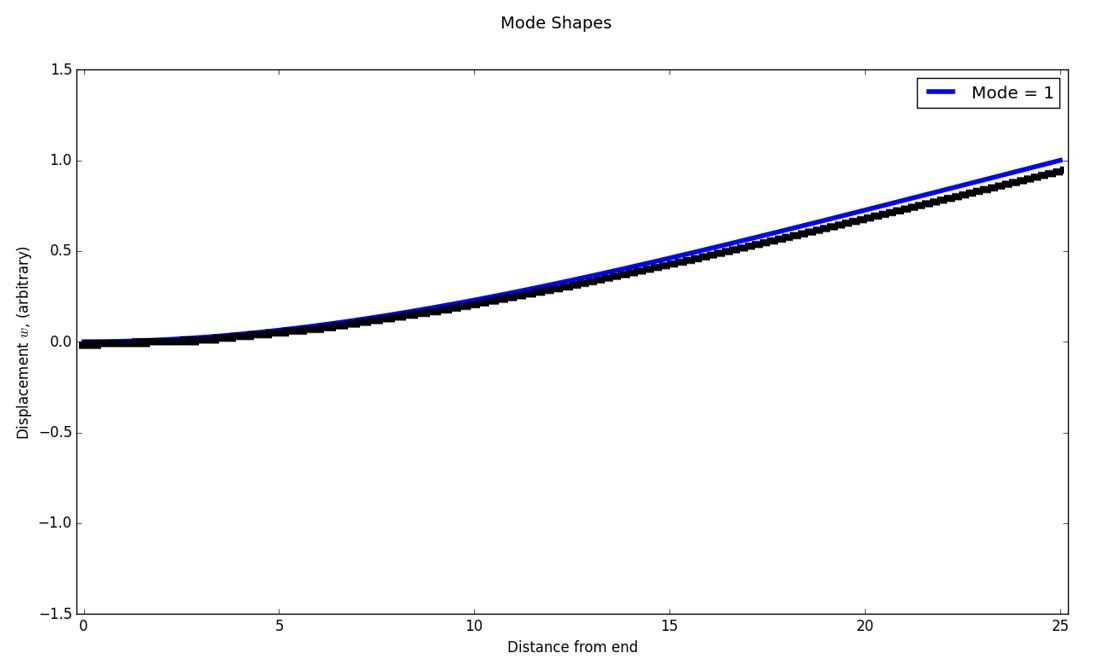
\includegraphics[height=4.70cm]{figures/F_1.jpg}
		\label{fig:F_1}
		}
		\quad
		\subfigure[Mode 2 ABAQUS and analytical comparison]
		{
		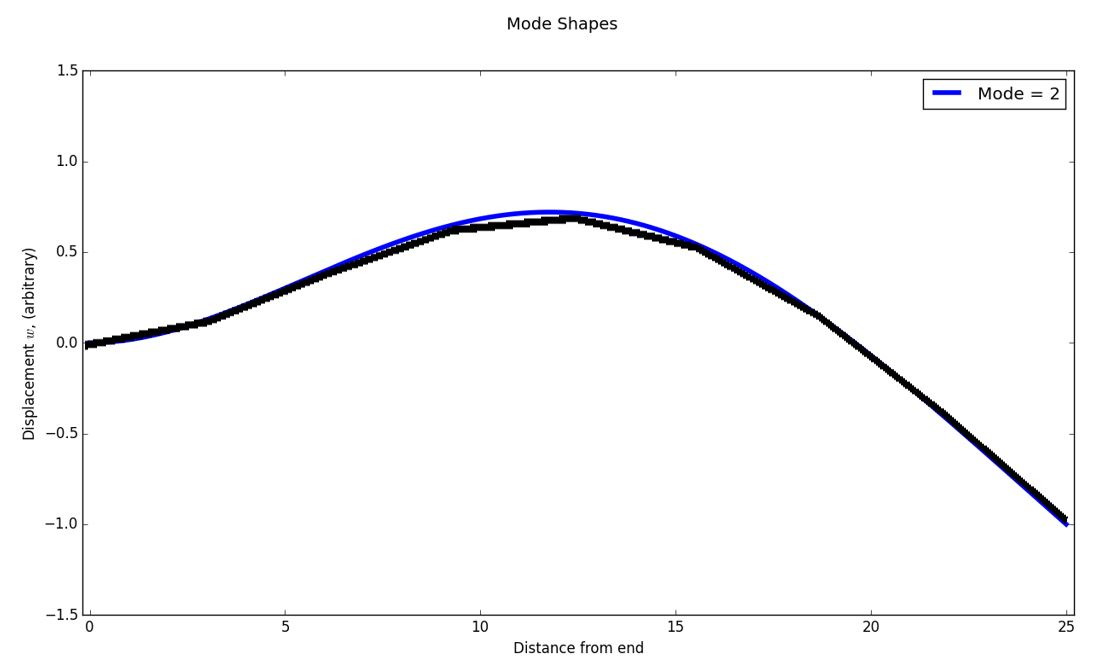
\includegraphics[height=4.70cm]{figures/F_2.jpg}
		\label{fig:F_2}
		}
		\quad
		\subfigure[Mode 3 ABAQUS and analytical comparison]
		{
		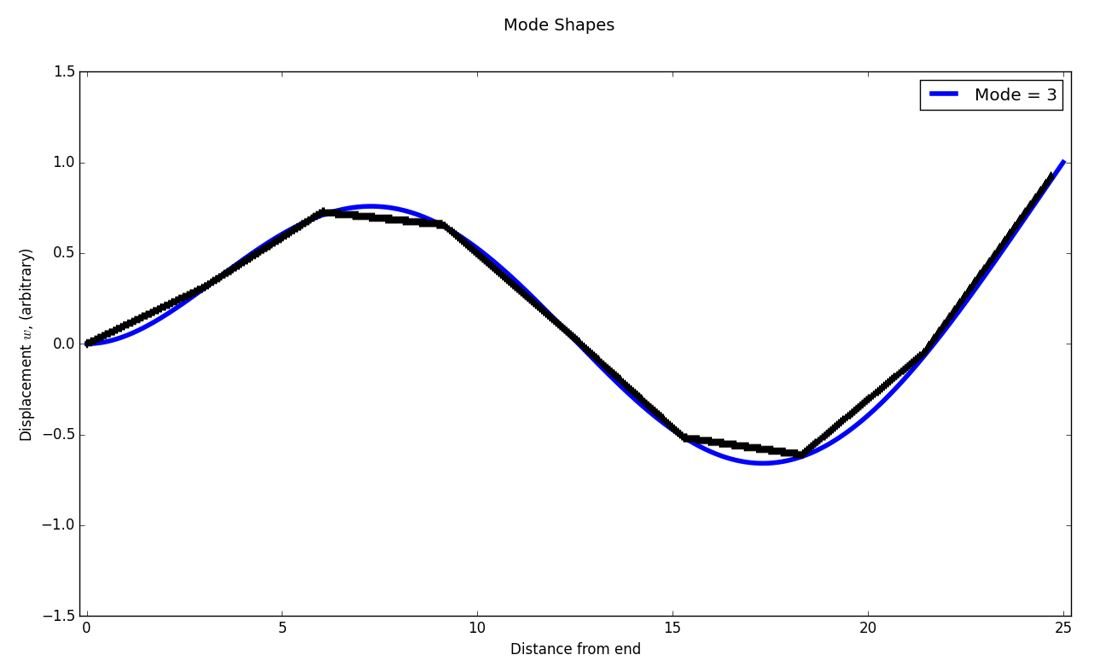
\includegraphics[height=4.70cm]{figures/F_3.jpg}
		\label{fig:F_3}
		}
		\quad
		\subfigure[Mode 4 ABAQUS and analytical comparison]
		{
		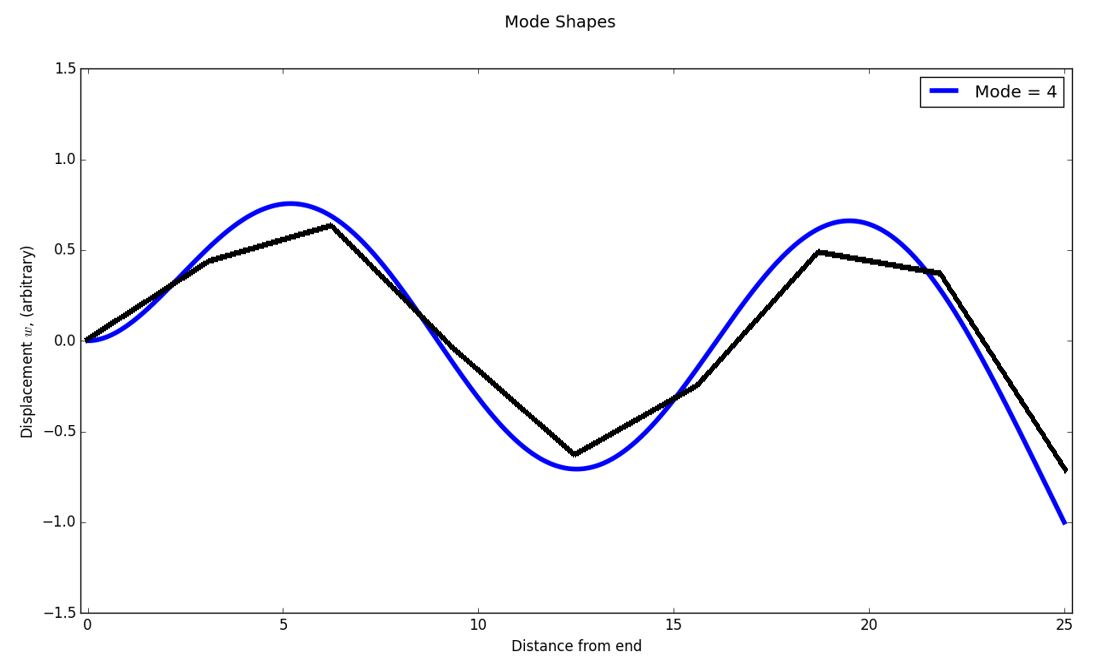
\includegraphics[height=4.70cm]{figures/F_4.jpg}
		\label{fig:F_4}
		}
		\caption{Modes 1 THRU 4}
		\label{fig:Modes14}
	\end{figure}
%

%
	\begin{figure}[H]
		\centering
		\subfigure[Mode 5 ABAQUS and analytical comparison]
		{
		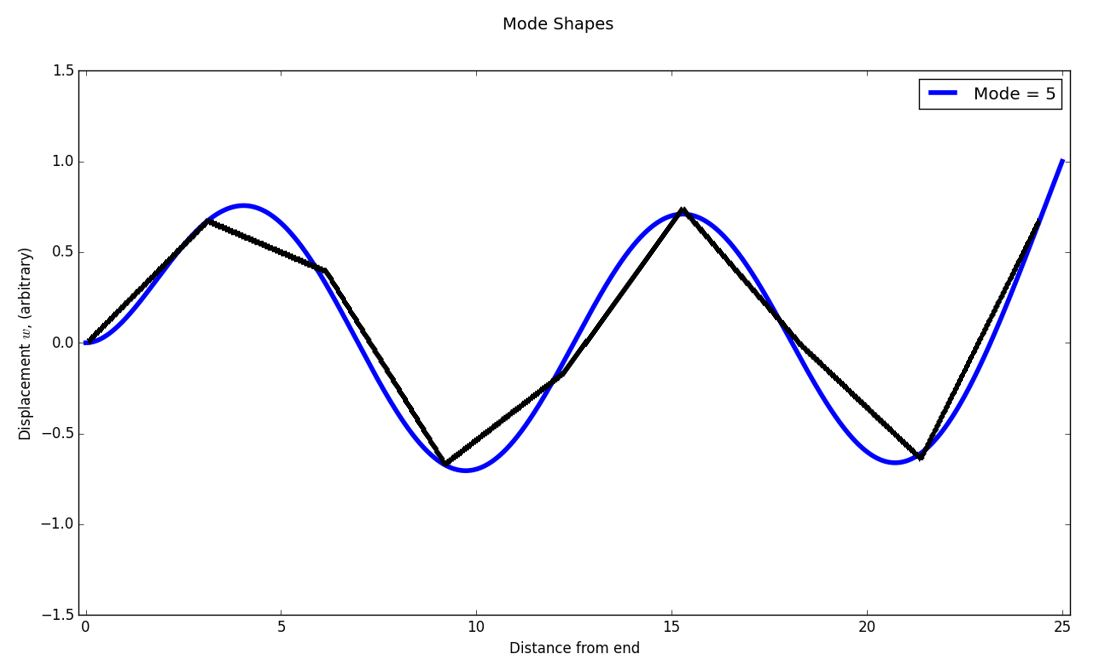
\includegraphics[height=4.70cm]{figures/F_5.jpg}
		\label{fig:F_1}
		}
		\quad
		\subfigure[Mode 6 ABAQUS and analytical comparison]
		{
		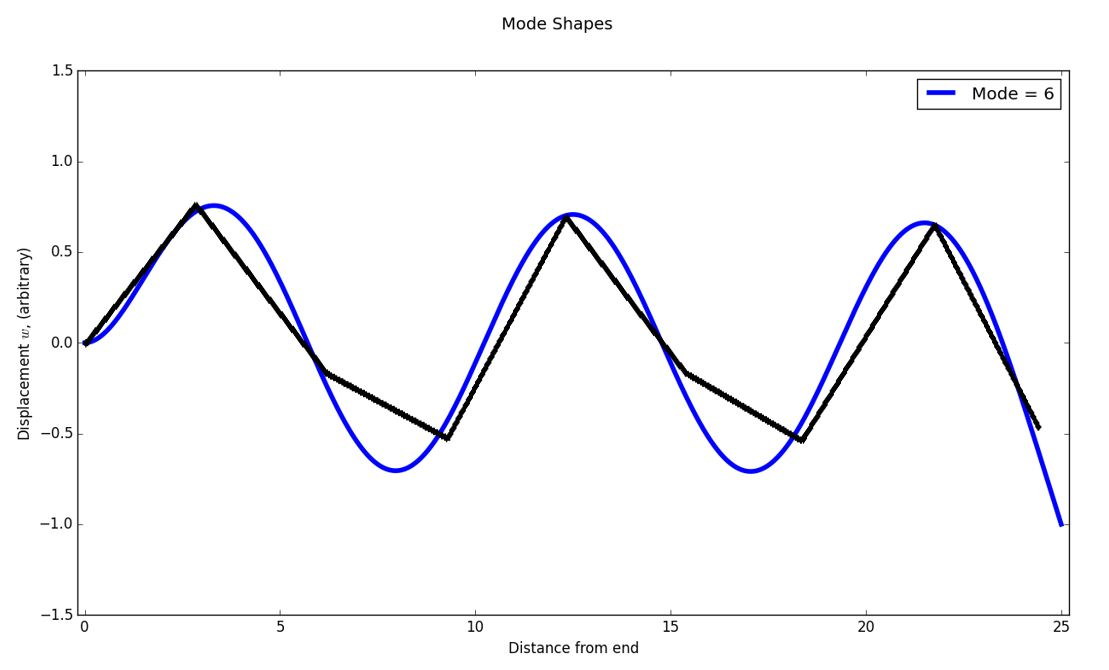
\includegraphics[height=4.70cm]{figures/F_6.jpg}
		\label{fig:F_2}
		}
		\quad
		\subfigure[Mode 7 ABAQUS and analytical comparison]
		{
		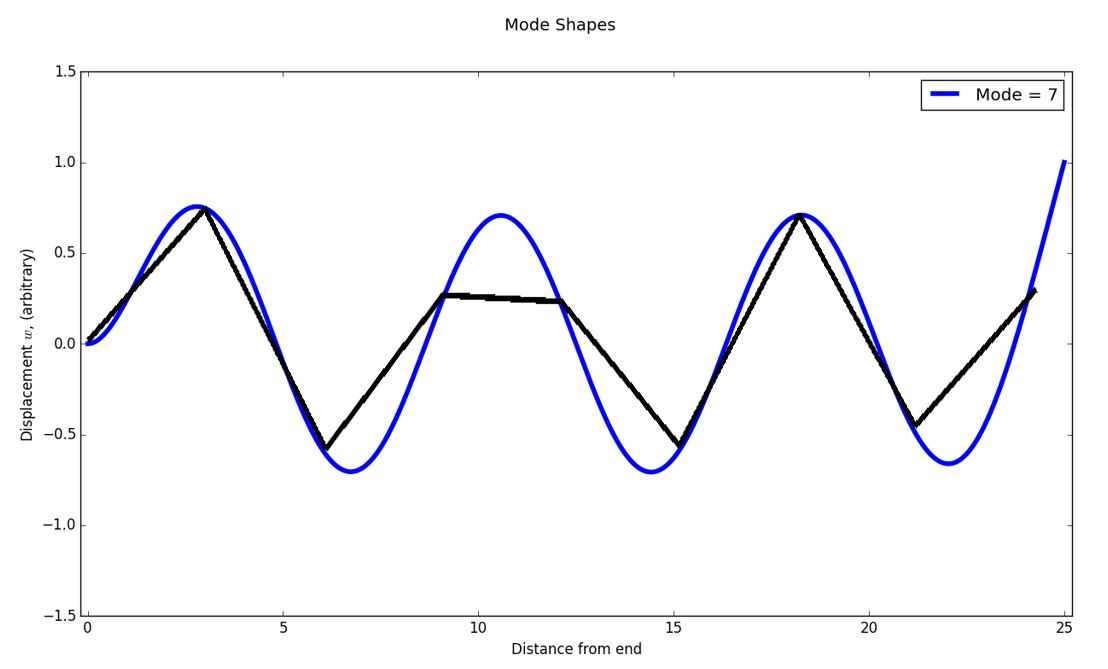
\includegraphics[height=4.70cm]{figures/F_7.jpg}
		\label{fig:F_3}
		}
		\quad
		\subfigure[Mode 8 ABAQUS and analytical comparison]
		{
		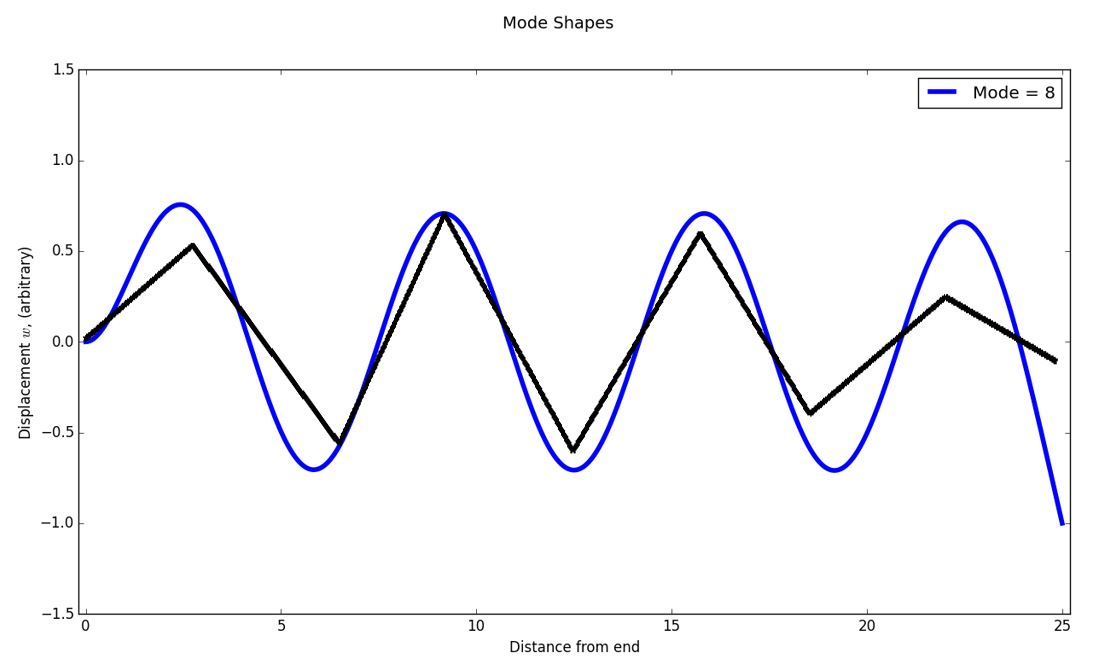
\includegraphics[height=4.70cm]{figures/F_8.jpg}
		\label{fig:F_4}
		}
		\caption{Modes 5 THRU 8}
		\label{fig:Modes58}
	\end{figure}
%

Next section compares analytical results to the 2 noded beam element coded in MATLAB.

\end{document}